Write a code chebfft2 for second-order differentiation by the FFT, and show by examples that it matches
the results obtained by matrices, apart from rounding errors.
\footnote{Again, this was not an assigned problem, however I did quite a bit of work for it and didn't
want to delete it.}\\\\

\begin{solution}\renewcommand{\qedsymbol}{}\ \\
    Here, we used the functions $\sin(x), e^x,$ and $e^{-x^2}$ as examples to demonstrate the chebfft2
    function. In order to write this function, all we needed to do is repeat the FFT, inverse FFT, and
    deriving the algebraic polynomial steps just on the derivative vector. So, we get the following
    graphs.

    \begin{figure}[htp]
        \centering
        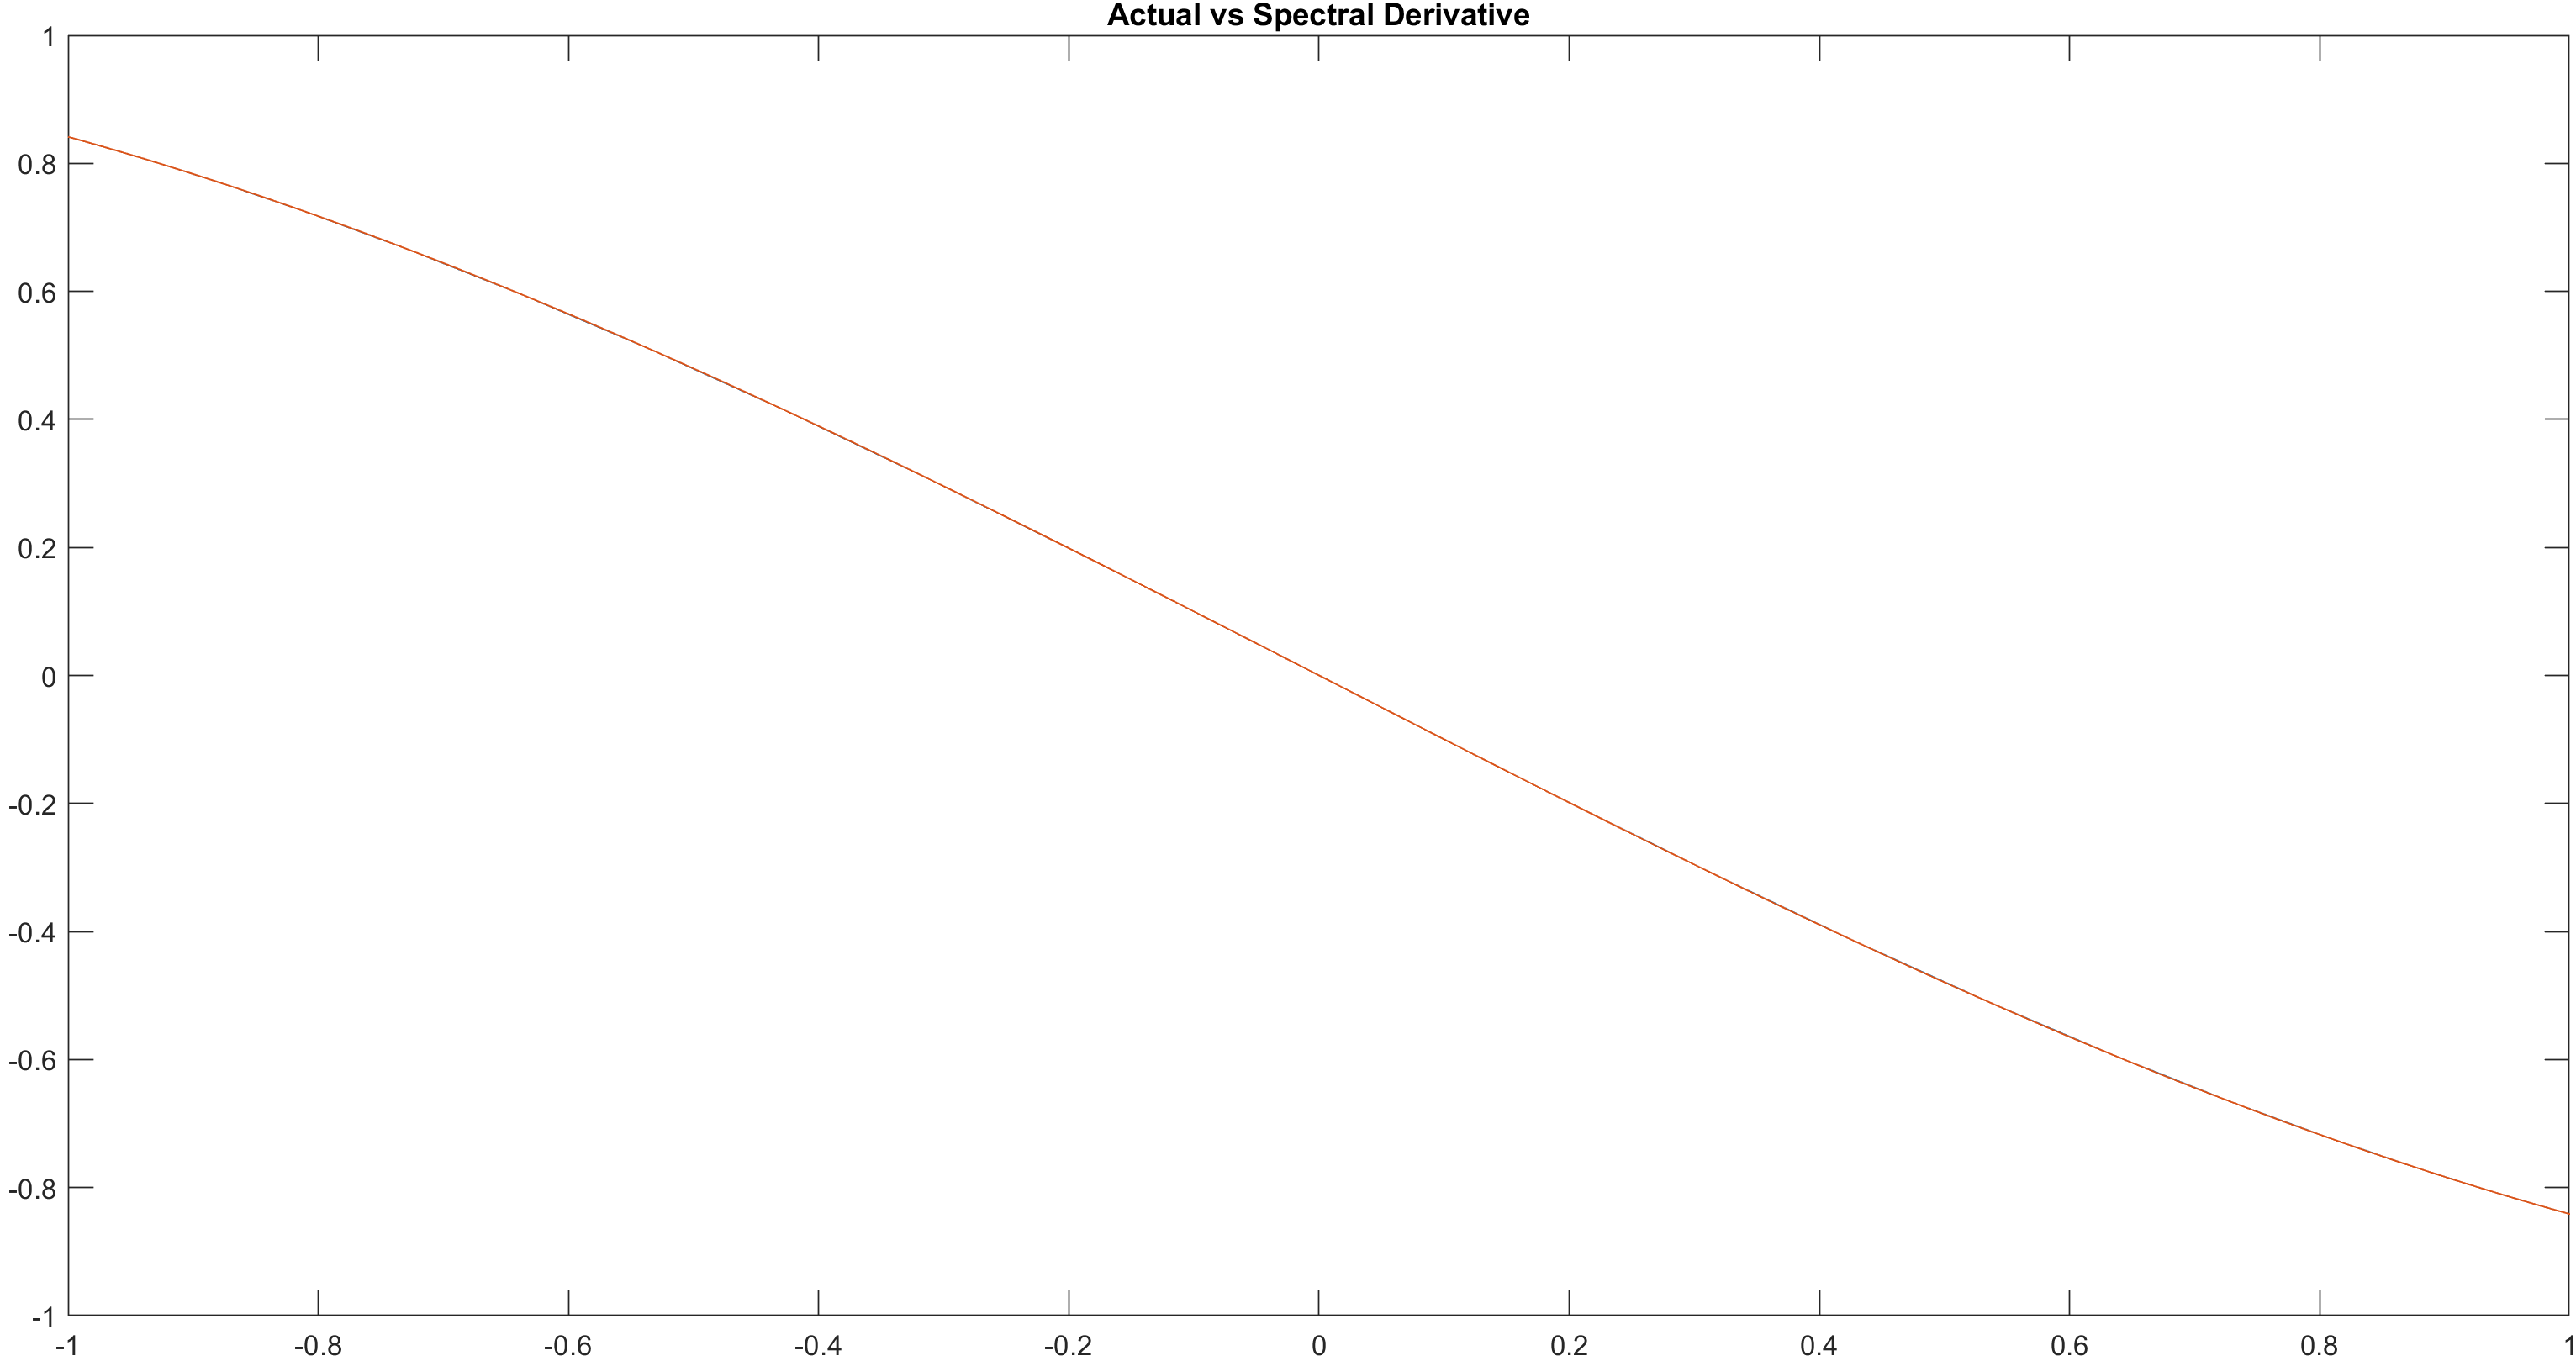
\includegraphics[scale=0.10]{8_5sin.PNG}
        \caption{$\sin(x)$}
    \end{figure}
    \begin{figure}[htp]
        \centering
        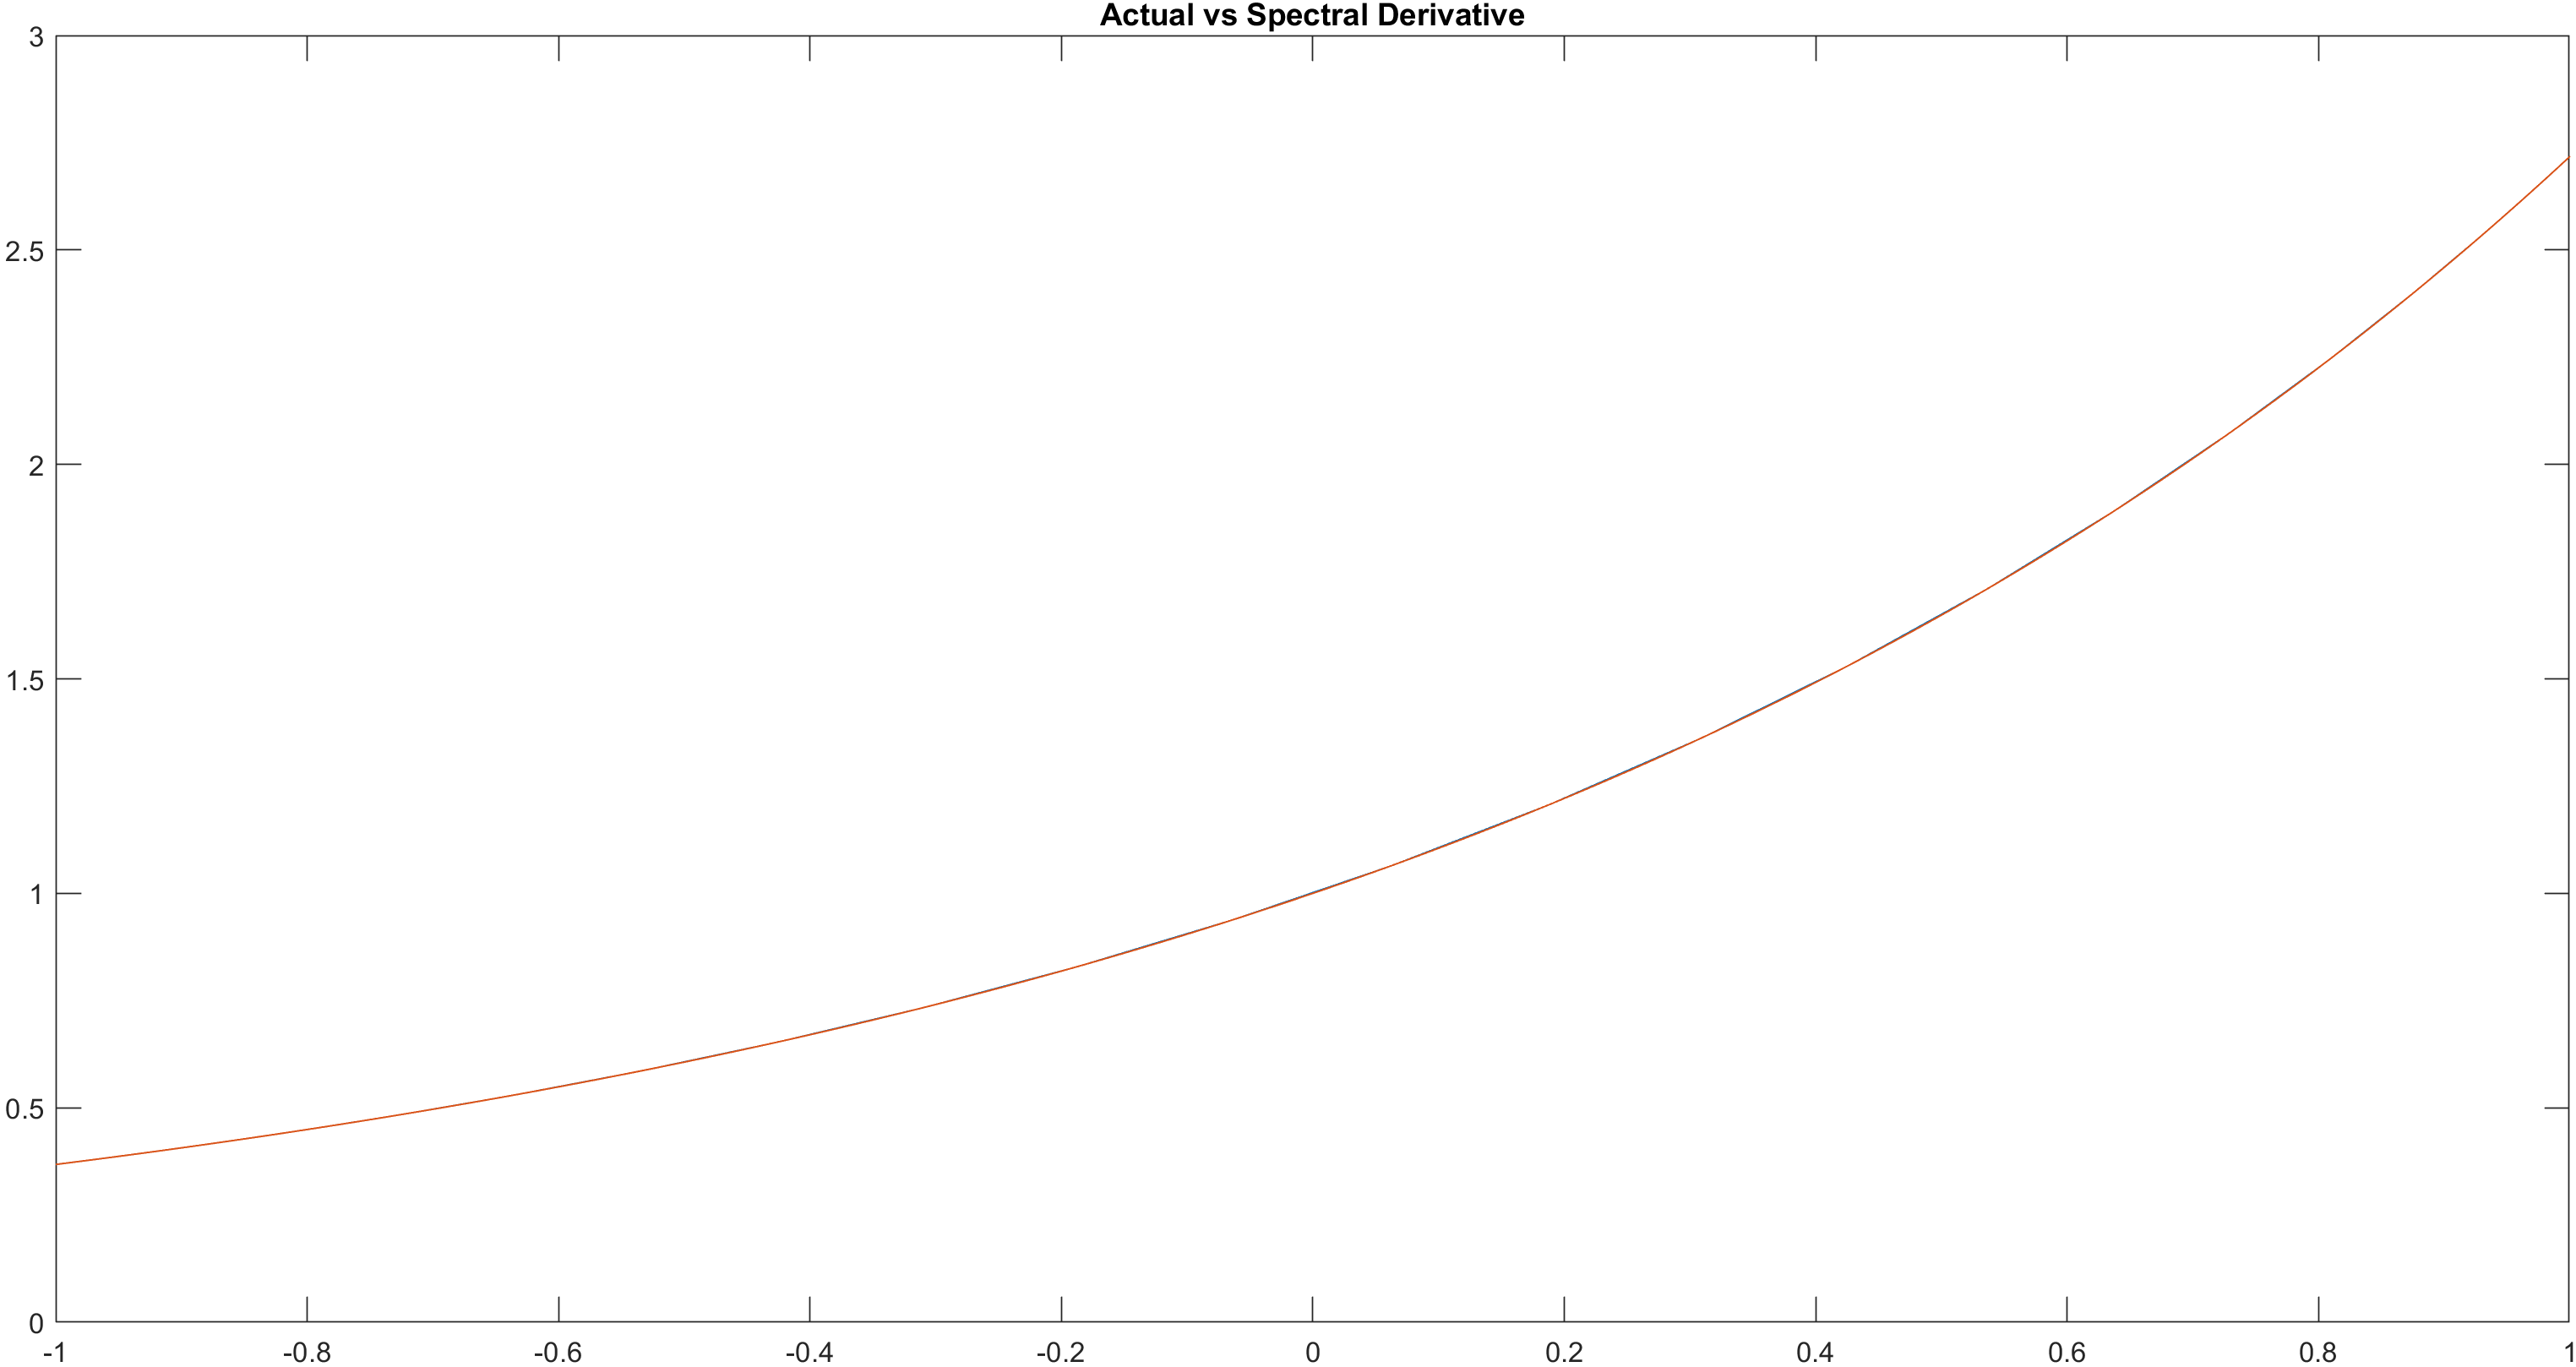
\includegraphics[scale=0.10]{8_5exp.PNG}
        \caption{$e^x$}
    \end{figure}
    \begin{figure}[htp]
        \centering
        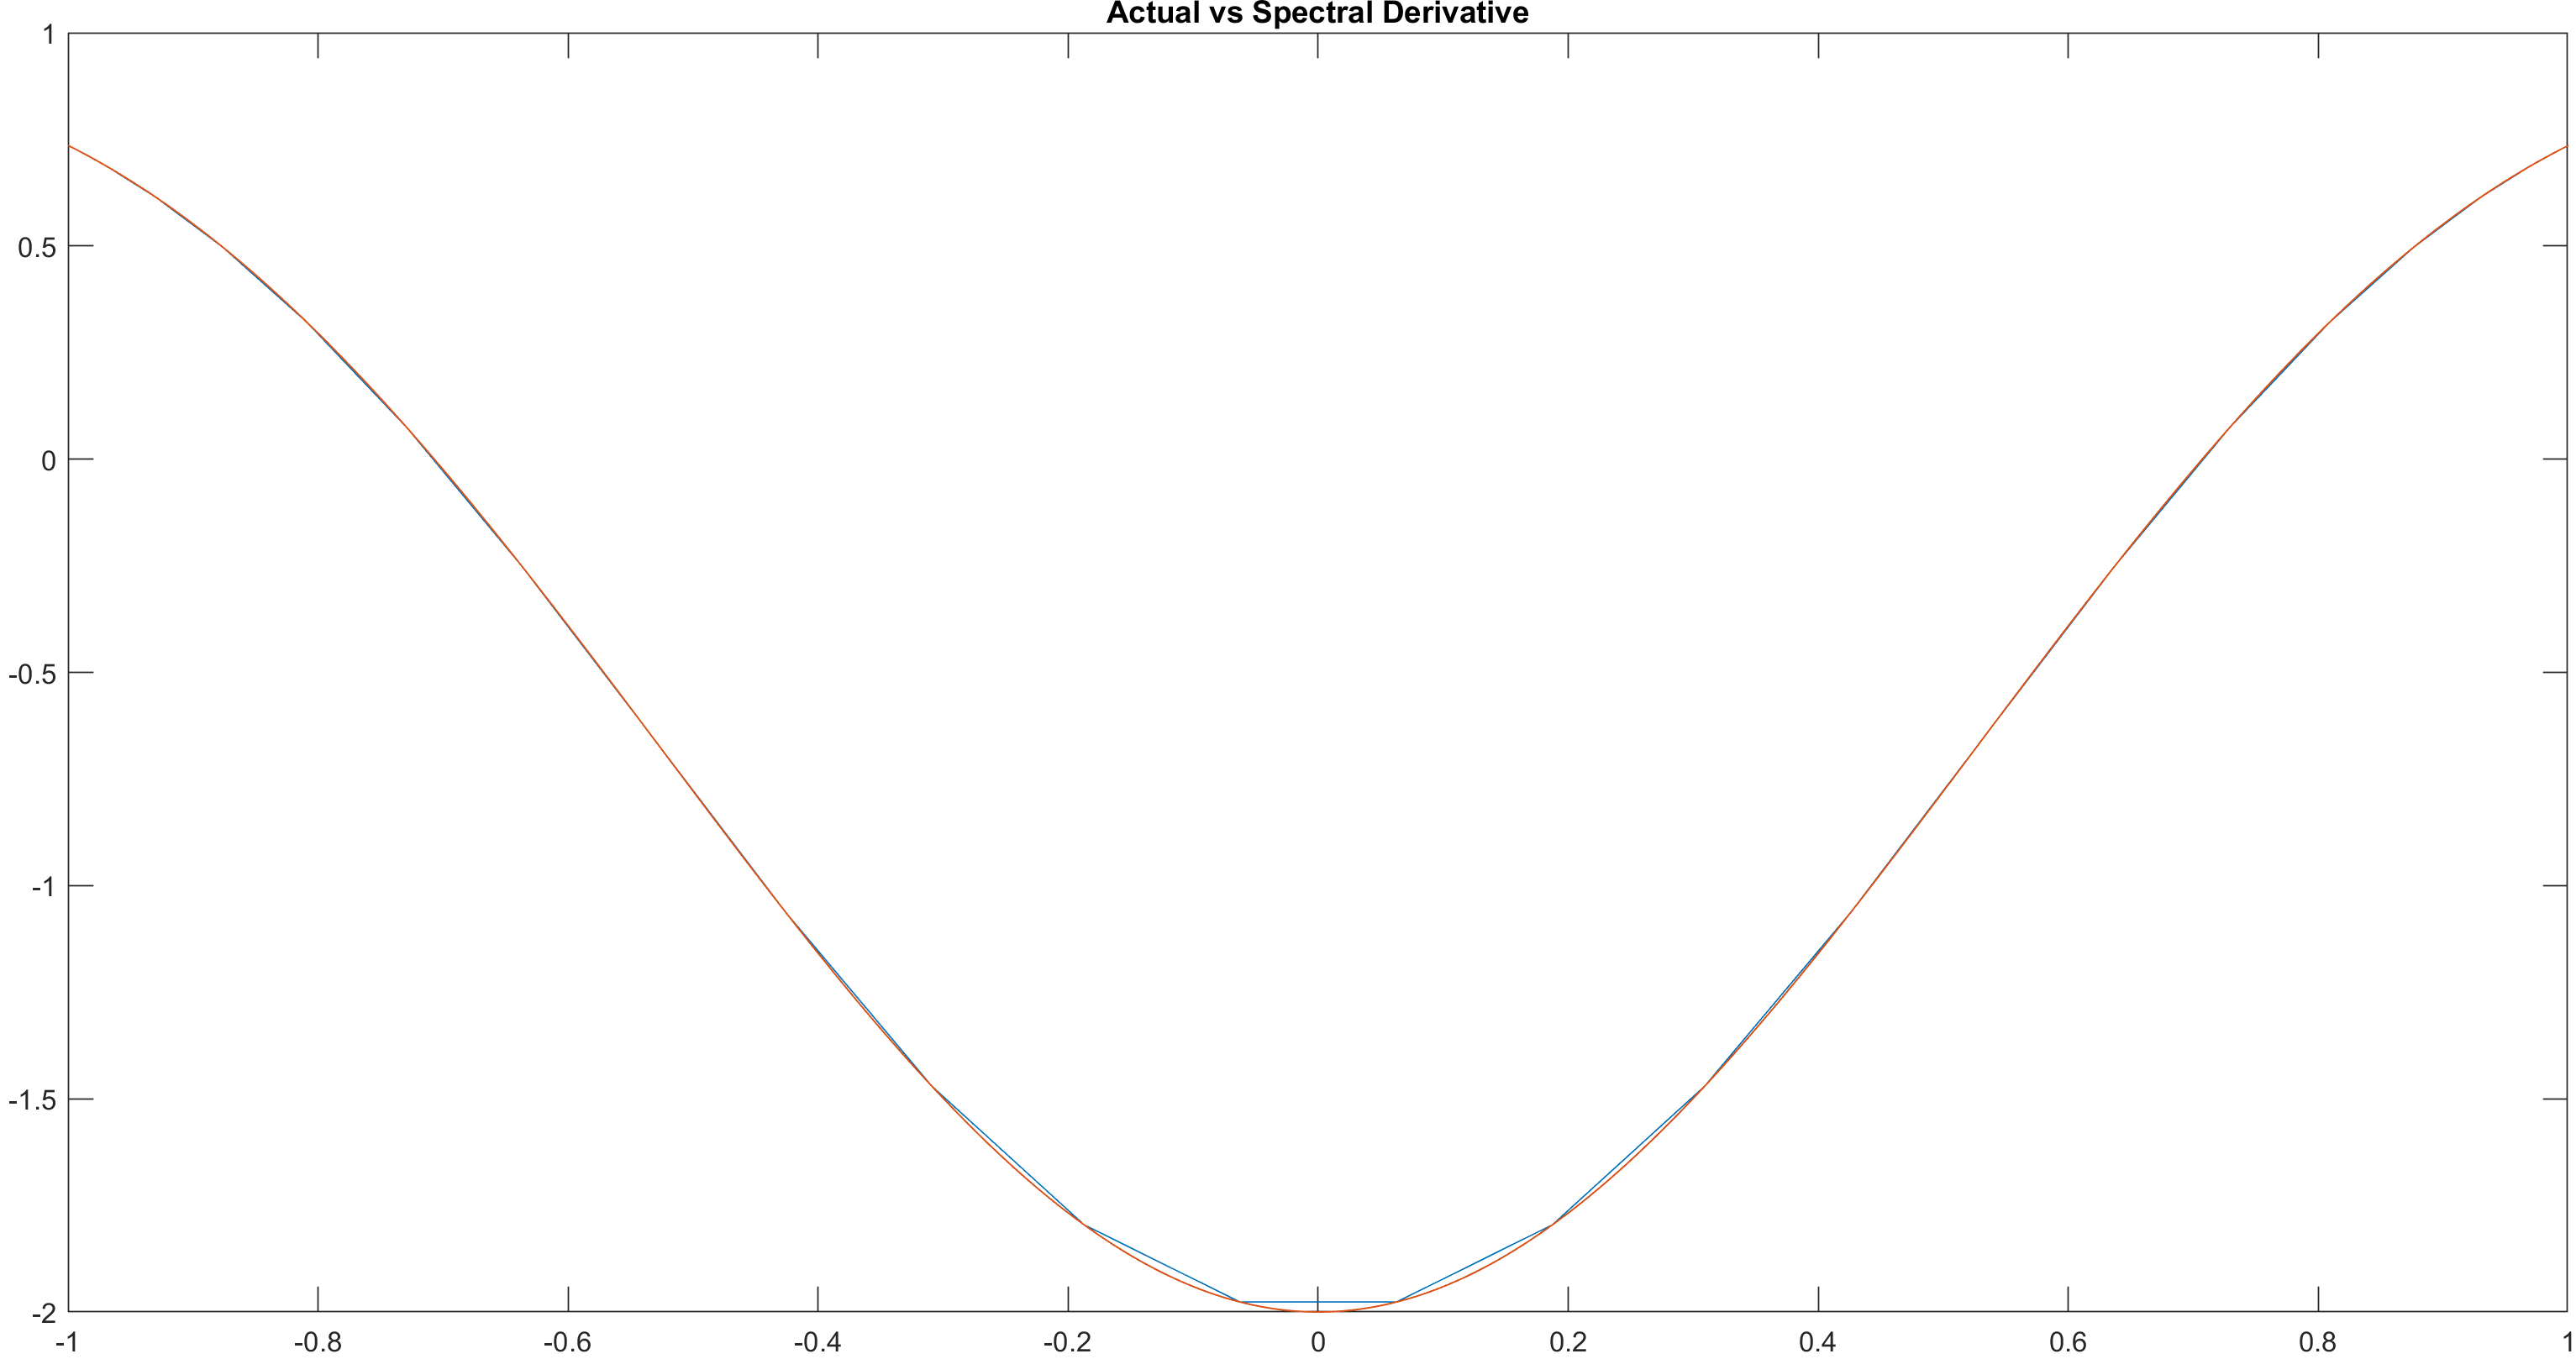
\includegraphics[scale=0.10]{8_5expx2.PNG}
        \caption{$e^{-x^2}$}
    \end{figure}

\end{solution}

\newpage
\lstinputlisting{problem8_6.m}